\section{Motivation}
\label{idea-sec-motivation}

IDEA's architecture is motivated by two observations. First, many sensor
network applications require a large portion of the network to meet their
fidelity requirements. As a result, failures of sensor nodes can deeply
impact delivered data quality. Indeed, the most heavily-loaded nodes are
often those that are most critical to the application. Consider a node near
the root of a spanning tree, which is responsible for forwarding traffic for
a substantial portion of the network. Loss of this single node can have a
disproportionate effect on the whole network's operation.

Second, in most applications, some portion of the load at each node is due to
interaction with other nodes and cannot be reduced unilaterally. In the case
of routing, nodes spend their own energy to listen to and forward packets for
other nodes. In such cases, load mitigation must be negotiated with the peer
nodes producing the load. For example, a node with a valuable sensor input
might do everything possible to reduce its own power consumption, but unless
it can move itself off of a high-traffic routing path, it will be unable to
reduce energy expenditure beyond a certain point.

Existing approaches to sensor network energy management suffer from several
weaknesses. Greedy approaches to local energy minimization assume that each
node minimizing its own power consumption is best for the network as a whole.
However, this is not always the case. Such approaches also cannot address the
external load problem described above. Some sensor network protocols embed
forms of distributed energy management into their operation, but by doing so
they encode policies unsuitable for certain applications. IDEA addresses
these deficiencies by providing a distributed service allowing any component
controlling distributed load to perform collaborative energy management.

\subsection{Example: Energy-Aware Routing}

\begin{figure}[t]
\begin{center}
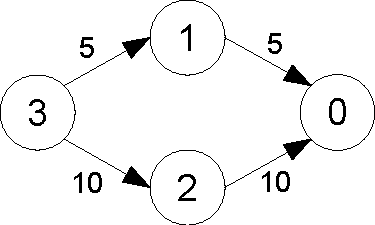
\includegraphics[width=0.6\hsize]{./5-idea/figs/motivationexample.pdf}
\end{center}
\caption{\textbf{Example routing problem.} The edges are the energy in mJ to
send a packet.}
\label{idea-fig-motivationexample}
\end{figure}

As a simple example demonstrating the need for IDEA, consider a four-node
routing problem. Figure~\ref{idea-fig-motivationexample} shows the network
topology, with the energy required to reliably transfer a packet over each
link shown. (To simplify the example we ignore receive costs, assume all
nodes have the same data rate of one packet per second, and assume a powered
sink.) The application attempts to localize events by collecting data from
the network, and must use all four nodes, meaning that the loss of a single
node will render the network useless.

Node~3 has two routes to the sink Node 0: $3,1,0$ and $3,2,0$. If Node~3
conserves power by making a local greedy decision, it will route through
Node~1, since sending a packet to Node~1 consumes $0.5$~mJ of energy as
opposed to $1.0$~mJ for sending to Node~2. Even assuming Node~3 knows the
power consumption of the links $1,0$ and $2,0$, with no other information it
still chooses the route though Node~1, which consumes less total energy per
packet than the route through Node~2, 1.0~mJ per packet versus 2.0~mJ.

The question we ask is, under what conditions will using route $3,1,0$ ---
which consumes the least energy locally and globally --- actually
\textit{harm} application performance?  We identify four situations where
using the alternative route $3,2,0$ is the correct choice, each described
below. To facilitate our discussion we define $B_n$, $C_n$ and $L_n$ as the
battery in joules, charging rate in mJ per second, and non-routing load in mJ
per second at Node $n$ respectively. The choice we are considering is between
two possible load distributions, $R \in \mathcal{R}$, where $R^{3,1,0} =
(0.0, 1.0, 1.0, 0.5)$ and $R^{3,2,0} = (0.0, 0.5, 2.0, 1.0)$. $R^{Route}_n$
represents the cost to Node $n$ assuming Node 3 uses the route indicated.
(Node~1 and Node~2 route directly to the sink.)  For example, $R^{3,2,0}_2$
is 2.0 mJ because the cost to send a packet from Node~2 to Node~0 is 1.0 mJ
and Node~2 must send two packets, one from Node~3 as well as a packet from
the data generated locally at Node~2.

\begin{itemize}

\item \textbf{Differences in initial battery levels:} If the nodes are not
harvesting energy ($C_n = 0 \forall n$), no non-routing load exist ($L_n = 0
\forall n$), and Nodes~2 and~3 have significantly more energy than Node~1,
then routing through Node~2 will increase the lifetime of Node~1, which due
to its low battery level defines the lifetime of the entire network.
Specifically, if $B_2 > B_1 * 2$ and $B_3 > B_1 * 2$  then using $R^{3,2,0}$
will increase the lifetime of the network.

\item \textbf{Differences in non-routing load rates:} Assuming equal initial
energy availability and no harvesting, consideration of non-routing load
$L_n$ is similar to differences in battery sizes. Differences in non-routing
load rates between the nodes could be due to higher sampling rates or sensor
energy costs on various nodes. Assuming $B_n = \beta$ $\forall n$ and $C_n =
0$ $\forall n$, the result is similar: if $L_2 + 1.0 \le L_1 - 0.5$ and $L_3
+ 0.5 \le L_1 - 0.5$ then using $R^{3,2,0}$ will increase the network's
lifetime.

\item \textbf{Differences in charging rates:} If $C = [0.0, 2.0, 2.0, 2.0]$,
then both routes allow all nodes to continue to charge, but $R^{3,1,0}$ leads
to an aggregate charging rate of $4.0$~mJ/s whereas $R^{3,2,0}$ produces an
aggregate charging rate of only $2.5$~mJ/s, leaving $R^{3,1,0}$ the better
option. However, if $C = [0.0, 0.5, 2.0, 2.0]$, then the application must
choose between the lower aggregate charging rate of $1.5$~mJ/s but better
survivability of $R^{3,2,0}$ and the higher aggregate charging rate of
$2.5$~mJ/s but unsustainability of $R^{3,1,0}$. Since our application cannot
tolerate the loss of a single node, it chooses the lifetime of Node~1 over
charging at Nodes~2 and~3, and thus $R^{3,2,0}$. Note that if $C = [0, 0.5,
1.0, 1.0]$, then no $R \in \mathcal{R}$ leads to a non-zero charging rate and
the best route is $R^{3,1,0}$.

\item \textbf{Overcharging:} Assuming that the batteries at Nodes~2 and~3
have reached capacity, but Node~1 has not, if $R^{3,2,0}_2 > C_2$ and
$R^{3,2,0}_3 > C_3$ then using $R^{3,2,0}$ will either increase the charging
rate at Node 1, if it is charging, or increase its lifetime by reducing its
load if it is not. Either outcome is beneficial.

\end{itemize}

Making the correct decision at Node~3 in all four cases requires that it know
the load rates, charging rates, and battery levels at Nodes~1 and~2. IDEA
addresses this problem by distributing this information across the set of
affected nodes. The four cases above motivate several features in the IDEA
design. In general, the network may want to shift load \textit{towards} nodes
that have a great deal of stored energy, low load rates, high charging rates,
or charging energy currently going to waste, and \textit{away} from nodes
with low batteries, low charging rates, or that are already highly-loaded. In
cases where shifting load produces extra overall load for the network, as it
does above, changes in load distribution must be managed by the application
based on its own goals and requirements. Had our application above been able
to tolerate the loss of Node~1, it might have chosen to optimize charging at
Nodes~2 and~3 in the third example. Respecting these differences, IDEA is
designed to facilitate application-level input into its decision-making
process.
